\documentclass[12pt]{article}
\usepackage[utf8]{inputenc} 
\usepackage[french]{babel}
\usepackage{graphicx} \graphicspath{{./}}
\usepackage{amsmath,amssymb,amsthm} 
% \usepackage{algorithm,algorithmic}
\usepackage{caption}
\usepackage[left=3cm,right=3cm,top=2cm,bottom=2cm]{geometry}
\usepackage{url} 
\usepackage[T1]{fontenc} 
\usepackage{xcolor}
\usepackage{float}
\usepackage{listings}
\lstset{ %
language=C++,                % choose the language of the code
basicstyle=\footnotesize,       % the size of the fonts that are used for the code
numbers=left,                   % where to put the line-numbers
numberstyle=\footnotesize,      % the size of the fonts that are used for the line-numbers
stepnumber=1,                   % the step between two line-numbers. If it is 1 each line will be numbered
numbersep=5pt,                  % how far the line-numbers are from the code
backgroundcolor=\color{white},  % choose the background color. You must add \usepackage{color}
showspaces=false,               % show spaces adding particular underscores
showstringspaces=false,         % underline spaces within strings
showtabs=false,                 % show tabs within strings adding particular underscores
frame=single,           % adds a frame around the code
tabsize=2,          % sets default tabsize to 2 spaces
captionpos=b,           % sets the caption-position to bottom
breaklines=true,        % sets automatic line breaking
breakatwhitespace=false,    % sets if automatic breaks should only happen at whitespace
escapeinside={\%*}{*)}          % if you want to add a comment within your code
}

\renewcommand\thesection{\arabic{section}}
\newcommand\hsp{\hspace{1.0cm}}

\begin{document}
\begin{titlepage}
\begin{center}
\vspace*{3cm}
\textsc{\Large Rapport}\\[1.5cm]
\vspace{1cm}

% Title
	% \HRule \\ [0.4cm]
	{ \huge \bfseries TDP 5\\[0.4cm] }
	% \HRule \\ [1.5cm]
	{ \bfseries Factorisation LU\\[0.4cm] }
	% \HRule \\ [1.5cm]

\vspace{3cm}

% Author and supervisor
	\begin{minipage}{0.5\textwidth}
	    \begin{center} \large
	             Nicolas \textsc{Dubois}\\
	             Aurélien \textsc{Falco}\\
	    \end{center}
	\end{minipage}
	\\[2cm]
    \end{center}

\vspace*{4cm}
\begin{flushright}Date : \today\end{flushright}
\end{titlepage}


\section{Introduction} % (fold)
\label{sec:introduction}
Le but du projet était d'implémenter une factorisation LU, en répartissant les calculs sur plusieurs processus. 

% section introduction (end)

\section{Factorisation LU} % (fold)
\label{sec:factorisation_lu}

\subsection{Méthode} % (fold)
\label{sub:methode}

\begin{figure}[H]
\centering

\includegraphics[width=0.8\textwidth]{lu}
\caption{Décomposition LU right-looking}
\label{fig:lu}
\end{figure}

Pour ce projet, nous utilisons la factorisation LU right-looking, illustrée par la figure \ref{fig:lu}. Nous pouvons y voir une partie de la factorisation déjà effectuée (L et U). Ensuite, nous appliquons l'algorithme expliqué (de façon simplifié) en Fig. \ref{code:lu}.

\begin{figure}[H]
\begin{lstlisting}
for (j = 0; j < MIN(m,n); j+=nb)
		dgetf2(m-j, nb, A[j, j]);
		dtrsm(Lower, nb, n-j-nb+1, A[j, j], A[j, j+nb]);
		dgemm(m-j-nb, n-j-nb, nb, A[j+nb, j], A[j, j+nb], A[j+nb, j+nb]);
\end{lstlisting}
\caption{Décomposition LU (dgetrf)}
\label{code:lu}
\end{figure}
Sur $B$, de largeur $nb$, nous effectuons une décomposition LU (dgetf2 ou dgetrf par exemple, mais ici nous avons utilisé dgetf2, étant donné que $nb$ est censé être relativement petit). Puis nous pouvons exécuter un dtrsm sur $L_0$ et $C$, essayant de résoudre l'équation \ref{eq:dtrsm}, et affectant le résultat dans $U_1$. Enfin, nous effectuons un dgemm sur $L_1$, $U_1$ et $E$, effectuant l'opération décrite dans l'équation \ref{eq:dgemm}. Puis nous itérons et réexécutons la totalité de ce procédé sur $E'$

\begin{equation}
\label{eq:dtrsm}
L_0 \times X = C
\end{equation}

\begin{equation}
\label{eq:dgemm}
E' = E - L_1 * U_1
\end{equation}

\subsection{Parallélisme} % (fold)
\label{sub:parallelisme}

Pour paralléliser les calculs sur plusieurs processeurs, une méthode est de distribuer des blocs colonnes, de largeur $nb$, et ce en serpentin. Cela signifie que les blocs colonnes seront réparties comme indiqué en Fig. \ref{fig:serpentin}.

\begin{figure}[H]
\centering
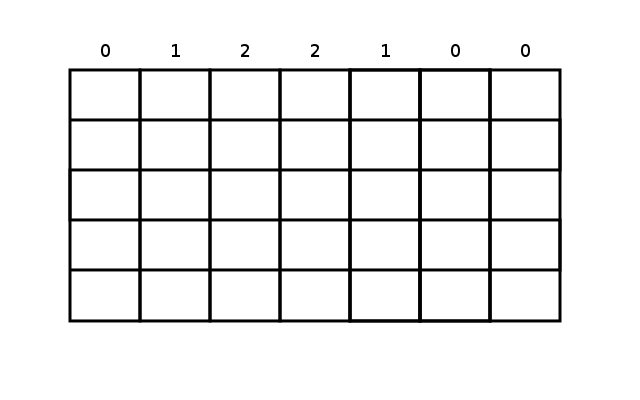
\includegraphics[width=0.8\textwidth]{serpentin}
\caption{Distribution en serpentin}
\label{fig:serpentin}
\end{figure}



\section{Exécution \& tests} % (fold)
\label{sec:execution}

Pour ce projet, nous avons effectué des tests de validation sur les fonctions algébriques, afin de s'assurer que celles-ci marchaient correctement, et pouvoir plus facilement isoler les problèmes. De même, le code a été segmenté pour permettre une lecture plus aisée de l'ordre dans lequel s'effectuent les diverses opérations. Afin de faciliter la mise en oeuvre de la factorisation par bloc, nous avons choisi de ne pas traiter les cas où la taille des blocs n'est pas multiple de la largeur et la longueur de la matrice.\\

Plusieurs fonctions intermédiaires ont été écrites afin de simplifier l'affichage, la génération ou encore la comparaison entre matrices (voir util.c et util.h).

Nous avons remarqué que pour des matrices de tailles croissantes, des erreurs d'arrondis apparaissaient et se propagaient rapidement. Ainsi, pour des matrices de taille $30 \times 30$, les erreurs commençaient à être significatives dans le calcul du dtrsm (de l'ordre de $0.1$). Nous n'avons pas remarqué ce genre d'erreurs dans les autres algorithmes toutefois, excepté dgesv qui utilise directement deux dtrsm. 

\section{Performances} % (fold)
\label{sec:perf}

Une série de tests est lancée sur différentes tailles de matrice ou différents nombres de processus plusieurs fois, afin d'obtenir des temps d'exécution moyens. Nous avons remarqué que l'algorithme passait beaucoup de temps dans les fonctions de répartition des données sur les processus (peu optimisées). Aussi avons-nous comparé les temps de calculs seulement. \\

La largeur des colonnes a été fixée à $64$, afin de pouvoir exécuter les calculs sur des matrices dont les tailles étaient des puissances de 2, pour simplifier la lecture des résultats. 
La Figure \ref{fig:sp-size} montre que plus les calculs sont importants, plus la parallélisation est effective.

\begin{figure}[H]
\centering
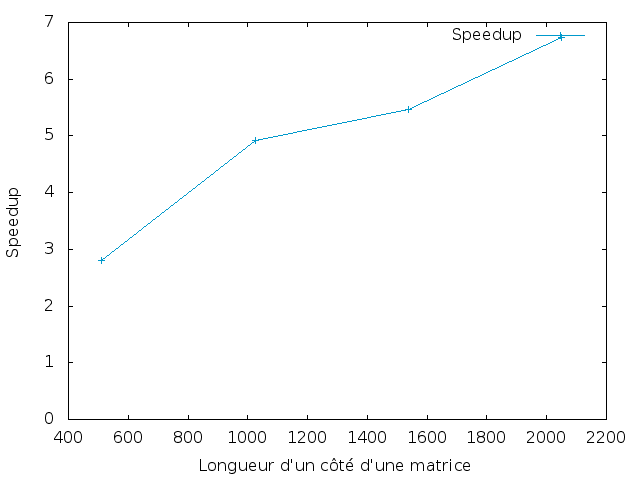
\includegraphics[width=0.8\textwidth]{sp-size.png}
\caption{Evolution du speedup avec la taille d'une matrice pour 8 processus}
\label{fig:sp-size}
\end{figure}

Comme l'indique la courbe de la Fig. \ref{fig:sp-proc}, le nombre de processeurs permet de réduire le temps d'exécution. Cette courbe a été tracée sur des matrices de dimensions $1024\times1024$. Nous pouvons remarquer que cette courbe est toujours inférieure à $y = x$. Le plateau ainsi que l'augmentation du speedup observés à 8 et 16 processus respectivement sont dûs à la taille des blocs utilisée pour les colonnes (64 doubles de largeur dans l'exemple). Nous avons alors 2 colonnes à calculer par processus à partir de 8 processus et ce chiffre descend à 1 colonne par processus lorsque $64*16 = 1024$. Pour profiter d'une accélération avec plus de processus, il faudrait diminuer la taille de des blocs. Il est également possible de séparer les blocs colonne en plusieurs blocs pour augmenter le parallélisme, qui s'amenuise au fil de l'algorithme (il y a peu de communication et beaucoup de calculs).

\begin{figure}[H]
\centering
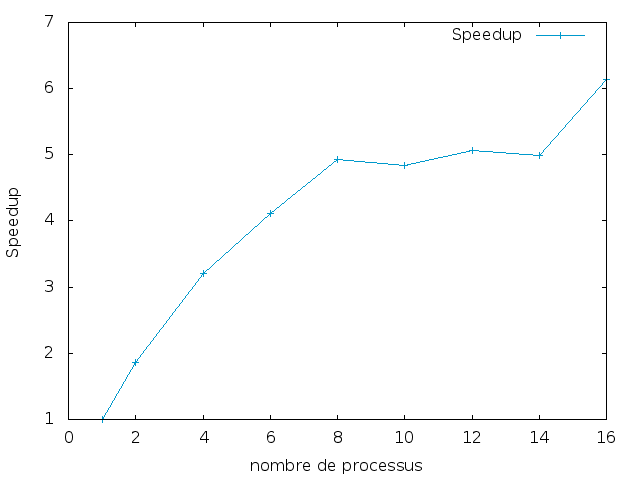
\includegraphics[width=0.8\textwidth]{sp-proc.png}
\caption{Accélération de notre programme par rapport au code séquentiel pour une matrice 1024x1024, en fonction du nombre de processeurs}
\label{fig:sp-proc}
\end{figure}

% section \ (end)



\end{document}
